\documentclass[a4paper, 12pt]{article}

\usepackage{tikz}
\usetikzlibrary{automata, positioning, arrows}
\usepackage{float}

\usepackage{xcolor}
\usepackage[left=2cm, right=2cm, top=2cm, bottom=2cm]{geometry}

\usepackage{ mathrsfs }

\usepackage{amsmath}

\tikzset{
	->,
	node distance=3cm, 
	>=stealth',
	every state/.style={thick},
	baseline}

\begin{document}
\pagenumbering{roman}
\title{
		\textbf{Group Members}\\ 
		Tevin Achong - 816000026\\
		Jimmel Greer - 816000045\\
		\textbf{Course Code:} COMP3602\\
		\textbf{Course Title:} Theory of Computing\\
		\textbf{Assignment:} 1
		\date{October 24, 2019}
}
\maketitle

\newpage
\begin{enumerate}

\item %1
\begin{itemize}
\item[(a)] $\{0^n \lor 1^m$ $|$ $n$ is even, $m$ is odd$\}$ ~\\

\begin{figure}[H]
	\centering
	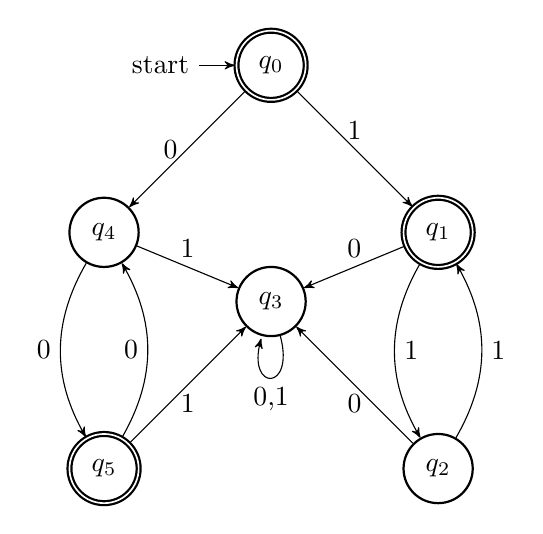
\begin{tikzpicture}
		
		\node[state, initial, accepting] (q0) {$q_0$};
		\node[state, accepting, below right of=q0] (q1) {$q_1$};
		\node[state, below of=q1] (q2) {$q_2$};
		\node[state, below of=q0] (q3) {$q_3$};
		\node[state, below left of=q0] (q4) {$q_4$};
		\node[state, accepting, below of=q4] (q5) {$q_5$};
		
		\draw 
		(q0) edge[above] node{1} (q1)
		(q0) edge[left] node{0} (q4)
		(q1) edge[bend right, right] node{1} (q2)
		(q1) edge[above] node{0} (q3)
		(q2) edge[bend right, right] node{1} (q1)
		(q2) edge[below] node{0} (q3)		
		(q3) edge[loop below, below] node{0,1} (q3)
		(q4) edge[above] node{1} (q3)
		(q4) edge[bend right, left] node{0} (q5)
		(q5) edge[bend right, left] node{0} (q4)
		(q5) edge[below] node{1} (q3)
		;
			
		
	\end{tikzpicture}
\end{figure}

\item[(b)] Any string that does not contain the substring 01 ~\\

\begin{figure}[H]
	\centering
	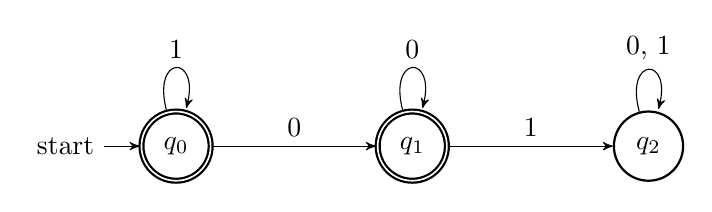
\begin{tikzpicture}
	
		\node[state, initial, accepting] (q0) {$q_0$};
		\node[state, accepting, right of=q0] (q1) {$q_1$};		 	
		\node[state, right of=q1] (q2) {$q_2$};
		
		\draw
		(q0) edge[loop above, above] node{1} (q1)
		(q0) edge[above] node{0} (q1)
		(q1) edge[loop above, above] node{0} (q1)
		(q1) edge[above] node{1} (q2)
		(q2) edge[loop above, above] node{0, 1} (q2)
		;
	
	\end{tikzpicture}
\end{figure}
\end{itemize}

\newpage
\item %2
\begin{itemize}
\item[(a)] Strings ending in 1011 ~\\

\begin{figure}[H]
	\centering
	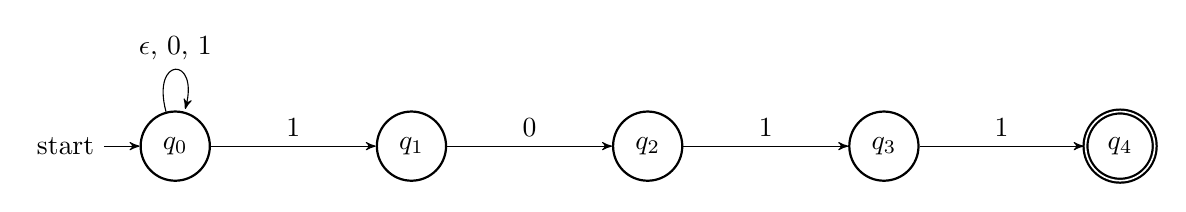
\begin{tikzpicture}
		\node[state, initial] (q0) {$q_0$};
		\node[state, right of=q0] (q1) {$q_1$};
		\node[state, right of=q1] (q2) {$q_2$};
		\node[state, right of=q2] (q3) {$q_3$};
		\node[state, accepting, right of=q3] (q4) {$q_4$};
		
		\draw
		(q0) edge[above] node{1} (q1)
		(q0) edge[loop above, above] node{$\epsilon$, 0, 1} (q1)
		(q1) edge[above] node{0} (q2)
		(q2) edge[above] node{1} (q3)
		(q3) edge[above] node{1} (q4)
		;
	\end{tikzpicture}
\end{figure}

\item[(b)] $\{101x101$ $|$ $x \in \Sigma^*\}$ ~\\
\begin{figure}[H]
	\centering
	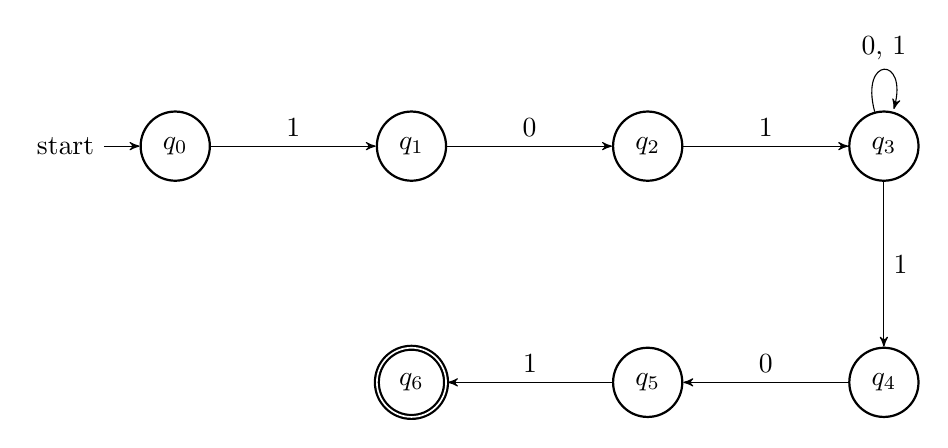
\begin{tikzpicture}
		\node[state, initial] (q0) {$q_0$};
		\node[state, right of=q0] (q1) {$q_1$};
		\node[state, right of=q1] (q2) {$q_2$};
		\node[state, right of=q2] (q3) {$q_3$};
		\node[state, below of=q3] (q4) {$q_4$};
		\node[state, left of=q4] (q5) {$q_5$};
		\node[state, accepting, left of=q5] (q6) {$q_6$};
		
		\draw
		(q0) edge[above] node{1} (q1)
		(q1) edge[above] node{0} (q2)
		(q2) edge[above] node{1} (q3)
		(q3) edge[right] node{1} (q4)
		(q3) edge[loop above, above] node{0, 1} (q3)
		(q4) edge[above] node{0} (q5)
		(q5) edge[above] node{1} (q6)
		;
	\end{tikzpicture}
\end{figure}

\item[(c)] $\{x(ab)^n$ $|$ $x \in \Sigma^*\, n$ is even\} ~\\
\begin{figure}[H]
	\centering
	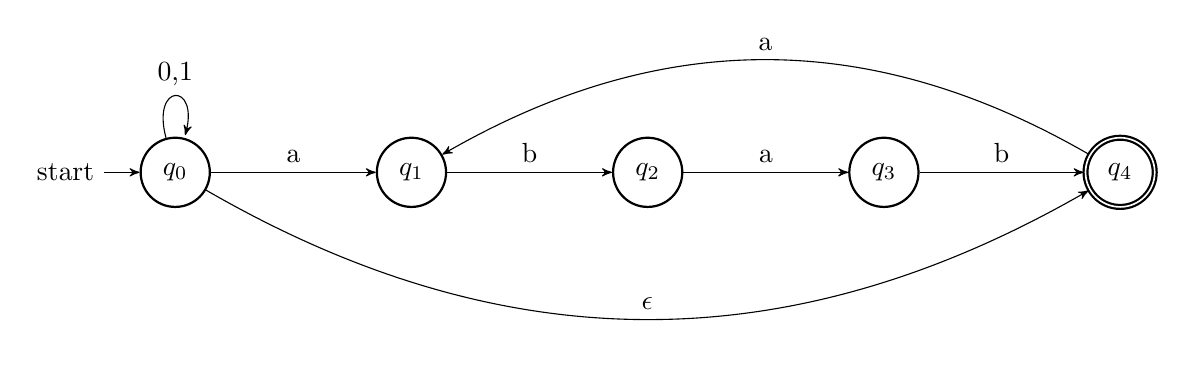
\begin{tikzpicture}
		\node[state, initial] (q0) {$q_0$};
		\node[state, right of=q0] (q1) {$q_1$};
 		\node[state, right of=q1] (q2) {$q_2$};
		\node[state,right of=q2] (q3) {$q_3$};
		\node[state, accepting, right of=q3] (q4) {$q_4$};

		\draw
		(q0) edge[loop above, above] node{0,1}(q1)
		(q0) edge[above] node{a} (q1)
		(q0) edge[bend right, above] node{$\epsilon$}(q4)
		(q1) edge[above] node{b} (q2)
		(q2) edge[above] node{a} (q3)
		(q3) edge[above] node{b} (q4)
		(q4) edge[bend right, above] node{a} (q1)
		;
	\end{tikzpicture}
\end{figure}

\end{itemize}

\newpage
\item %3
Let us refer to the DFA in Question 1b as $M$. Then 
$ M = \{\{q_0, q_1, q_2\}, \{0, 1\}, \delta, q_0, \{q_0, q_1\}\} $
where $ \delta $ is given by:\\
$\delta(q_0, 0) = q_1$\\
$\delta(q_0, 1) = q_0$\\
$\delta(q_1, 0) = q_1$\\
$\delta(q_1, 1) = q_2$\\
$\delta(q_2, 0) = q_2$\\
$\delta(q_2, 1) = q_2$\\
 
\item %4
Let us refer to the NFA in Question 2b as $N$. Then 
$ N = \{\{q_0, q_1, q_2, q_3, q_4, q_5, q_6\}, \{0, 1\}, \delta, q_0, \{q_6\}\} $
where $ \delta $ is given by:\\
$\delta(q_0, 0) = \{\}$\\
$\delta(q_0, 1) = \{q_1\}$\\
$\delta(q_0, \epsilon) = \{\}$\\
$\delta(q_1, 0) = \{q_2\}$\\
$\delta(q_1, 1) = \{\}$\\
$\delta(q_1, \epsilon) = \{\}$\\
$\delta(q_2, 0) = \{\}$\\
$\delta(q_2, 1) = \{q_3\}$\\
$\delta(q_2, \epsilon) = \{\}$\\
$\delta(q_3, 0) = \{q_3\}$\\
$\delta(q_3, 1) = \{q_3, q_4\}$\\
$\delta(q_3, \epsilon) = \{\}$\\
$\delta(q_4, 0) = \{q_5\}$\\
$\delta(q_4, 1) = \{\}$\\
$\delta(q_4, \epsilon) = \{\}$\\
$\delta(q_5, 0) = \{\}$\\
$\delta(q_5, 1) = \{q_6\}$\\
$\delta(q_5, \epsilon) = \{\}$\\
$\delta(q_6, 0) = \{\}$\\
$\delta(q_6, 1) = \{\}$\\
$\delta(q_6, \epsilon) = \{\}$\\

\newpage
\item ~\\ %5
\textbf{Key/Legend:}\\ 
{\color{blue} $\rightarrow$ \$0.05}\\
{\color{olive} $\rightarrow$ \$0.10}\\
{\color{magenta} $\rightarrow$ \$0.25}\\
{\color{red} $\rightarrow$ \$1.00}

\begin{figure}[H]
	\centering
	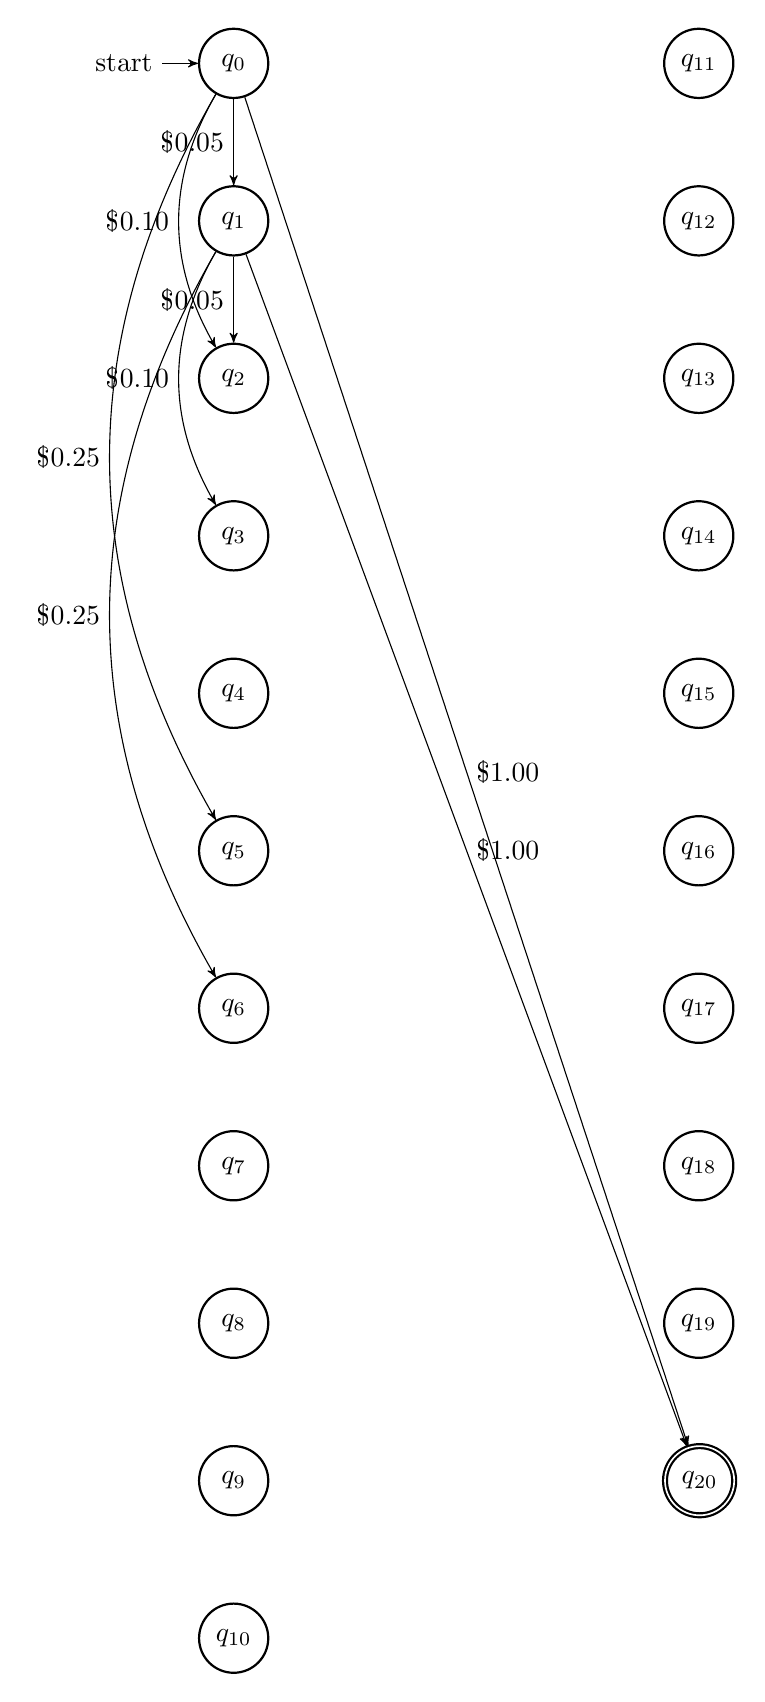
\begin{tikzpicture}[node distance=2cm]
		%LHS
		\node[state, initial] (q0) {$q_0$};
		\node[state, below of=q0] (q1) {$q_1$};
		\node[state, below of=q1] (q2) {$q_2$};
		\node[state, below of=q2] (q3) {$q_3$};
		\node[state, below of=q3] (q4) {$q_4$};
		\node[state, below of=q4] (q5) {$q_5$};
		\node[state, below of=q5] (q6) {$q_6$};
		\node[state, below of=q6] (q7) {$q_7$};
		\node[state, below of=q7] (q8) {$q_8$};
		\node[state, below of=q8] (q9) {$q_9$};
		\node[state, below of=q9] (q10) {$q_{10}$};
		
		%RHS
		\node[state, right=2.3cm and 5cm of q0] (q11) {$q_{11}$};
		\node[state, right=2.3cm and 5cm of q1] (q12) {$q_{12}$};
		\node[state, right=2.3cm and 5cm of q2] (q13) {$q_{13}$};
		\node[state, right=2.3cm and 5cm of q3] (q14) {$q_{14}$};
		\node[state, right=2.3cm and 5cm of q4] (q15) {$q_{15}$};
		\node[state, right=2.3cm and 5cm of q5] (q16) {$q_{16}$};
		\node[state, right=2.3cm and 5cm of q6] (q17) {$q_{17}$};
		\node[state, right=2.3cm and 5cm of q7] (q18) {$q_{18}$};
		\node[state, right=2.3cm and 5cm of q8] (q19) {$q_{19}$};
		\node[state, accepting, right=2.3cm and 5cm of q9] (q20) {$q_{20}$};
		
		\draw
		(q0) edge[left] node{\$0.05} (q1)
		(q0) edge[bend right, left] node{\$0.10} (q2)
		(q0) edge[bend right, left] node{\$0.25} (q5)
		(q0) edge[right] node{\$1.00} (q20)
		
		(q1) edge[left] node{\$0.05} (q2)
		(q1) edge[bend right, left] node{\$0.10} (q3)
		(q1) edge[bend right, left] node{\$0.25} (q6)
		(q1) edge[right] node{\$1.00} (q20)
		
		
		;
	\end{tikzpicture}
\end{figure}

\newpage
\item ~\\ %6



\begin{figure}[H]
	\centering
	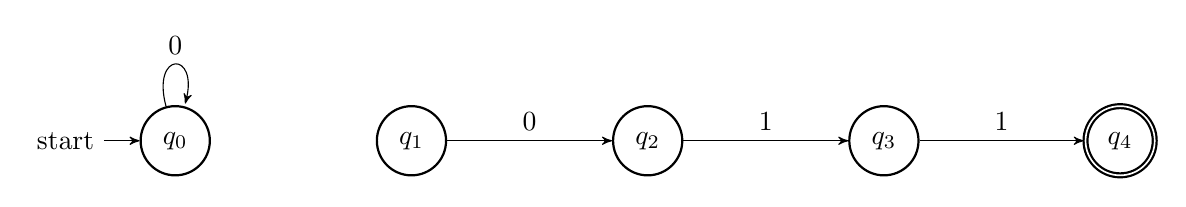
\begin{tikzpicture}
		\node[state, initial] (q0) {$q_0$};
		\node[state, right of=q0] (q1) {$q_1$};
		\node[state, right of=q1] (q2) {$q_2$};
		\node[state, right of=q2] (q3) {$q_3$};
		\node[state, accepting, right of=q3] (q4) {$q_4$};
		
		\draw
%		(q0) edge[above] node{1\\0} (q1)
		(q0) edge[loop above, above] node{0} (q1)
		(q1) edge[above] node{0} (q2)
		(q2) edge[above] node{1} (q3)
		(q3) edge[above] node{1} (q4)
		;
	\end{tikzpicture}
\end{figure}

\item %7
$\mathscr{L}_{1} - \mathscr{L}_{2}$ can be expressed as $(\mathscr{L}_{1} \bigcup \mathscr{L}_2) \bigcap \overline{\mathscr{L}_{2}}$, assuming they are within the same universal set. This defines set difference in terms of intersection, union and complement, for which the regular languages are known to be regular. Thus it can be concluded that $\mathscr{L}_{1}  - \mathscr{L}_{2}$ is a regular language.  




\item %8

\item ~\\%9
\begin{center}
	\begin{tabular}{|c|c|c|}
	\hline
	\textbf{Regular Expression} & \textbf{Recognized Strings} & \textbf{Non-Recognized Strings}\\
	\hline
	$a^*b^*$ & &\\
	\cline{2-3}
	& &\\
	\hline
	$a(ba)^*bb$ & &\\
	\cline{2-3}
	& &\\
	\hline
	$a^+ \cup b^*$ & &\\
	\cline{2-3}
	& &\\
	\hline
	$(\epsilon \cup a)b$ & &\\
	\cline{2-3}
	& &\\
	\hline
	\end{tabular}
\end{center}
\end{enumerate}


\pagenumbering{arabic}
\end{document}